\documentclass[11pt]{article}
 
\usepackage[margin=1in]{geometry} 
\usepackage{amsmath,amsthm,amssymb}
\usepackage{graphicx} 


\newcommand{\N}{\mathbb{N}}
\newcommand{\Z}{\mathbb{Z}}
 
\newenvironment{problem}[2][Problem]{\begin{trivlist}
\item[\hskip \labelsep {\bfseries #1}\hskip \labelsep {\bfseries #2.}]}{\end{trivlist}}
\newenvironment{lemma}[2][Lemma]{\begin{trivlist}
\item[\hskip \labelsep {\bfseries #1}\hskip \labelsep {\bfseries #2.}]}{\end{trivlist}}
\newenvironment{exercise}[2][Exercise]{\begin{trivlist}
\item[\hskip \labelsep {\bfseries #1}\hskip \labelsep {\bfseries #2.}]}{\end{trivlist}}

\newenvironment{question}[2][Question]{\begin{trivlist}
\item[\hskip \labelsep {\bfseries #1}\hskip \labelsep {\bfseries #2.}]}{\end{trivlist}}
\newenvironment{corollary}[2][Corollary]{\begin{trivlist}
\item[\hskip \labelsep {\bfseries #1}\hskip \labelsep {\bfseries #2.}]}{\end{trivlist}}

\usepackage{indentfirst}
\linespread{1.2}     % 调整间距
\setlength{\parindent}{0pt}

\begin{document}

 
% --------------------------------------------------------------
%                         Start here
% --------------------------------------------------------------
 
\title{Homework 3 DS-GA 1002 }%replace X with the appropriate number
\author{Yuhao Zhao\\ %replace with your name
N17578783} %if necessary, replace with your course title
 
\maketitle
\begin{problem}{1}
\end{problem}
(a) Since the delivery points are uniformly distributed, $f(x,y)  = \frac{1}{26}$ for  (x,y) $\in [0,13] \times [0,2]$\\
Let D be the deliver distance. The company is located ate the center i.e (6.5,1). \\
$E(D) = \int_{0}^{6.5} \int_{0}^{1} |x - 1|+|y-6.5|dxdy \\$
By symmetry, $E(D) = 4 \int_{0}^{6.5} \int_{0}^{1} (6.5 -x + 1 - y) \frac{1}{26} dy dx = \frac{4}{26} \int_{0}^{6.5} [y(6.5 - x +1) - \frac{y^2}{2}] |_{y=0}^1 dx$\\
$=\frac{4}{26} \int_{0}^{6.5} 6.5 - x +1 - \frac{1}{2}dx = 3.75$ \\

(b) Since we know that the distance is a non-negative random variable, the probability that the messenger has to travel more than 5 miles by Markov is: 
$P(D \geq 5) \leq \frac{E(D)}{5} = \frac{3.75}{5} = 75\%$

\begin{problem}{2}
\end{problem}
 (a) Since we need to have at least 100lb X or 100lb R, given X $\in$ [0,100], R is uniformly distributed over [100,300], given X $\in$ [100,300], R is uniformly distributed over [0,300]. X and R are symmetric. $f((x,y)\in ([0,100]\times [100,300]) \cup ([100,300] \times [0,300])) = \frac{1}{80000}$
 % \\P((x,y) \in [100,300]\times [0,100]) = \frac{1}{6}, f(x,y) = \frac{1}{6} \frac{1}{20000} \\P((x,y) \in [100,300]\times [100,300]) = \frac{2}{3}  ,f(x,y) = \frac{2}{3} \frac{1}{40000}$ 

 \begin{center}
 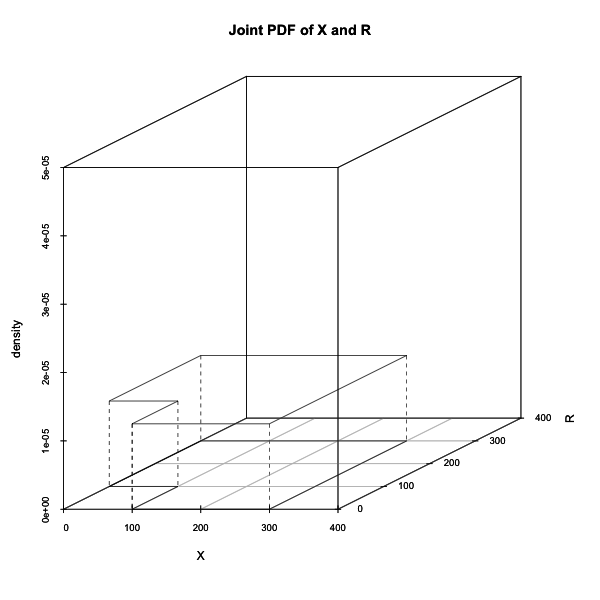
\includegraphics[height = 3.30in]{Q2_a}
 \end{center}
 
  (b) Since $Cov(X,R) = E(XR) - E(X)E(R)$\\
  $f_x(x) =\int_{R} f_{x,r}(x,r)dr = \frac{1}{400} (0<x<100), $and $  \frac{3}{800} (100<x<300)$\\
  $E(X) = \int_{0}^{300} xf_x(x)dx = \int_{0}^{100} \frac{x}{400}dx +\int_{100}^{300} \frac{3x}{800}dx = 162.5$\\
  By symmetry, $E(R) = E(X)  = 162.5$\\
  $E(XR) =\int_{100}^{300} \int_{0}^{100} XR  \frac{1}{80000}dXdR +\int_{0}^{300} \int_{100}^{300} XR  \frac{1}{80000}dXdR\\
   = \frac{10000}{4} + \frac{90000}{4} = 25000$\\
  $ E(X)E(R) =26406.25 \neq E(XR)$, Therefore, $E(XR) - E(X)E(R) \neq 0$.\\ X and R are correlated.\\
    
  
  (c) Since X and R are correlated, they are not independent. \\
  In particular, one counterexample is that, $P(Y = 20|X = 20) = 0 \neq P(Y = 20)$\\
  
  \begin{question}{3}
  	\end{question}
  (a) The assumption for this statement to be true is that, the number of customer and the money spend by each customer should be independent. \\
  Let X be the number of customers every night, and Y be the total money the customers spend every night. \\
  We know that: $E(X) = 40$, and $E(Y) = 30$\\
  
  (b) let the probability of having a good night be P, and the average number of customers is 40\\
  we have $p \times 100 + (1-P)\times 10 = 40 $, $P = \frac{1}{3}$\\
  
  (c) $E(Y)  = E(E(Y|X)) = \frac{1}{3} \times10 + \frac{2}{3} \times 40 = 30$\\
  
  (d) $E(XY) = E(E(XY|Y)) = E(XE(X|Y)) = 100 \times 10 \times \frac{1}{3} + 10\times 40\times \frac{2}{3} = \frac{1000}{3} +\frac{800}{3} = 600$\\
  This a counterexample to the management's statement. In this case on average, 40 customers visit the restaurant, and each customer spends 30 dollars. But actually, the restaurant makes 600  dollars per night. \\ 
  
  \begin{question}{4}
  \end{question}
  
  (a) Let X be the price of copper and Y be the amount of stock. $E(XY)  = 2 \times 10^6, X \leq 5,Y \leq 0.5 \times 10^6$. By the information given, we can only use the Markov inequality to bound $P(XY < 1)$.\\
  $P(XY<10^6) = 1 - P(XY > 10^6) <\frac{E(XY)}{10^6} = 2$, we have $P(XY >10^6 ) > -1$. This means the Markov yield no useful information. \\
  Another approach is that we consider the largest probability$\tilde{p}$ which makes the mean still be 2M. Since XY $\leq$ 2.5, this requires: $\tilde{P}(XY<1)\times 1 +(1- \tilde{P}(XY>1))2.5 = 2, \tilde{P}(XY<1) = \frac{1}{3}$\\
  Therefore, the upper bound is $\frac{1}{3}$
  
  (b) The price of copper and the amount of copper should be dependent. When the price is high, traders tend to sell more copper and thus the amount of copper in stock should be low.\\
  
  (c) By Chebyshev inequality: $P(|XY - E(XY)| \geq10^6) \leq \frac{Var(XY)}{10^{12}}$\\ 
  We assume independence, $Var(XY) =E(X^2)E(Y^2) - E^2(X)E^2(Y) = (Var(X)+E^2(X))(Var(Y) + E^2(Y)) -E^2(X)E^2(Y) = Var(X)Var(Y) +E^2(Y)Var(X) +E^2(X)Var(Y) $\\
  $E(Y) = \frac{E(XY)}{E(X)} = \frac{4*10^6}{9}$\\
 $ Var(X)Var(Y) = 0.2^2 \times 10^8 = 4 \times 10^6$ \\
 $Var(XY)  =   4 \times 10^6 + \frac{16*10^{12}}{81} \times  0.04 + 4.5^2 \times 10^8 \approx 9.93 *10^{9}$\\
  $P(|XY - 2\times 10^6| \geq10^6) \leq \frac{9.93 *10^{9}}{10^{12}} \approx 9.93\times 10^{-3}$\\
  Since XY $\leq$ 2.5$\times 10^6$ ,$P(XY \geq 3\time 10^6) = 0$\\
   $P(|XY - 2\times 10^6| > 10^6) = P(XY<10^{6}) \leq 9.93\times 10^{-3}$
  
   \begin{question}{5}
   \end{question}
  (a) $Var(Y| X = x)$ is a function of x. It represents the variance of Y given a certain value of X = x, it maps every x to a real number.\\
  
  (b) $Var(Y|X)$ is a random variable($\sigma $ field). \\
  
  (c) $Var(Y) = E(Y^2) - E^2(Y) = E(E(Y^2|X)) - E^2(E(Y|X)) \\=E(E(Y^2|X)) -E(E^2(Y|X)) +E(E^2(Y|X))  - E^2(E(Y|X))\\ = E(Var(Y|X))+E(E^2(Y|X))  - E^2(E(Y|X)) \\=  E(Var(Y|X)) + Var(E(Y|X)) $\\
  This law indicates that: the variance of Y is composed of (1) the average of the variance of Y about the Y values based on X, as X varies, and (2) the variance of the Y expectation based on X, as X varies\\
  
  (d)  Let Y be the time at which a runner gets injured, X be the age of the player\\
  $Y|X<30 \sim exp(1) , Y|X>30 \sim exp(2), P(X >30) = 0.2$, The mean and var of exp is $\frac{1}{\lambda}, \frac{1}{\lambda^2}$\\
  
  $E(Y) = E(E(Y|X)) = 0.8 \times \frac{1}{1} + 0.2 \times \frac{1}{2} = 0.9$\\
  
  $Var(Y) = E(Var(Y|X)) + Var(E(Y|X))\\
   E(Var(Y|X))  = 0.8 \times \frac{1}{1^2} + 0.2 \times \frac{1}{2^2}$\\
   $E(Y|X)$ is a random variable of X, $E(Y|X) = 1 $ with p =0.8 and $E(Y|X) = \frac{1}{2} $with P = 0.2\\
   $Var(E(Y|X)) = E(E^2(Y|X)) - E^2(Y) = 0.8 \times 1 + 0.2 \times \frac{1}{4}  - 0.9^2 = 0.04$\\
   $Var(Y) = 0.85 + 0.04  = 0.89$\\
   $std(Y) = \sqrt{0.89}$
    
\end{document}